% Residual-Based Certification and Adaptive Approximation of Solution Operators
% Martin Eigel, WIAS Berlin
% Working draft — started 2026-06-20

\documentclass[a4paper,11pt]{article}

%% ── Packages ────────────────────────────────────────────────────────────────
\usepackage[utf8]{inputenc}
\usepackage[T1]{fontenc}
\usepackage[english]{babel}
\usepackage{amsmath,amssymb,amsthm}
\usepackage{mathtools}
\usepackage{bm}
\usepackage{stmaryrd}% for \mathbbm
\usepackage{mathrsfs}
\usepackage{enumerate}
\usepackage{hyperref}
\usepackage{cleveref}
\usepackage{color}
\usepackage{graphicx}
\usepackage{algorithm}
\usepackage{algpseudocode}
\usepackage[margin=3cm]{geometry}
\usepackage{cite}
\usepackage{booktabs}

%% ── Theorem environments ────────────────────────────────────────────────────
\theoremstyle{plain}
\newtheorem{theorem}{Theorem}[section]
\newtheorem{lemma}[theorem]{Lemma}
\newtheorem{proposition}[theorem]{Proposition}
\newtheorem{corollary}[theorem]{Corollary}
\newtheorem{assumption}[theorem]{Assumption}

\theoremstyle{definition}
\newtheorem{definition}[theorem]{Definition}
\newtheorem{example}[theorem]{Example}
\newtheorem{remark}[theorem]{Remark}
\newtheorem{algorithmbox}[theorem]{Algorithm}

%% ── Operators ───────────────────────────────────────────────────────────────
\DeclareMathOperator{\KL}{KL}
\DeclareMathOperator{\rank}{rank}
\DeclareMathOperator{\diam}{diam}
\DeclareMathOperator{\osc}{osc}
\DeclareMathOperator{\argmin}{arg\,min}
\DeclareMathOperator{\argmax}{arg\,max}
\DeclareMathOperator{\supp}{supp}
\DeclareMathOperator{\dist}{dist}
\DeclareMathOperator{\Span}{span}
\DeclareMathOperator{\trace}{tr}
\DeclareMathOperator{\Var}{Var}
\DeclareMathOperator{\Cov}{Cov}
\renewcommand{\Pr}{\mathbb{P}}
\newcommand{\E}{\mathbb{E}}

%% ── Shortcuts ───────────────────────────────────────────────────────────────
\newcommand{\R}{\mathbb{R}}
\newcommand{\N}{\mathbb{N}}
\newcommand{\calG}{\mathcal{G}}
\newcommand{\calV}{\mathcal{V}}
\newcommand{\calM}{\mathcal{M}}
\newcommand{\calU}{\mathcal{U}}
\newcommand{\calX}{\mathcal{X}}
\newcommand{\calY}{\mathcal{Y}}
\newcommand{\calA}{\mathcal{A}}
\newcommand{\calB}{\mathcal{B}}
\newcommand{\wh}{\widehat}
\newcommand{\wt}{\widetilde}
\newcommand{\eps}{\varepsilon}
\newcommand{\dd}{\,\mathrm{d}}
\newcommand{\inner}[2]{\langle#1,#2\rangle}
\newcommand{\norm}[1]{\|#1\|}
\newcommand{\abs}[1]{|#1|}
\newcommand{\one}{\mathbbm{1}}

%% ── Title ───────────────────────────────────────────────────────────────────
\title{Residual-Based Certification and Adaptive Approximation\\of Solution Operators}
\author{Martin Eigel\thanks{Weierstrass Institute for Applied Analysis and Stochastics (WIAS), Berlin. \texttt{martin.eigel@wias-berlin.de}}}
\date{}

\begin{document}

\maketitle

\begin{abstract}
We develop a rigorous framework for the certified adaptive approximation of solution operators for parametric elliptic PDEs. 
Given a family of uniformly coercive operators $\{A_y\}_{y\in U}$, we consider the solution map $\calG:U\to V$, $y\mapsto u(y)$ where $A_y(u(y))=f_y$.
For an approximate operator $\wh\calG_n$, we define the \emph{operator residual} $R_n(y)=f_y-A_y(\wh\calG_n(y))$ and show that the Bochner-space error $\|\calG-\wh\calG_n\|_{L^2_\mu(U;V)}$ is bounded by the dual norm of the residual (reliability).
We combine this with a weak-greedy enrichment strategy that achieves convergence rates matching the Kolmogorov $n$-widths of the operator manifold, and a Monte Carlo estimator of the residual norm that provides a statistical certificate with high probability.
The main result (Theorem~\ref{thm:certified}) is a certified weak-greedy operator approximation theorem: under uniform coercivity, width decay, and statistical residual estimation, the adaptive algorithm achieves
\[
\|\calG-\wh\calG_n\|_{L^2_\mu(U;V)} \le C n^{-s} + C\sum_{k\ge n}\delta_k,
\]
where $n^{-s}$ is the width decay rate and $\delta_k$ is the statistical estimation error.
The framework is architecture-independent and is demonstrated for polynomial chaos operator approximations of affine-parametric diffusion problems, where the certificate tracks the true error within a factor~1 and the Monte Carlo estimator converges at the predicted $O(M^{-1/2})$ rate.
The limitations of the framework are illustrated in a regime of slow parametric decay, where the operator manifold has poor Kolmogorov width decay and enrichment stalls.
This provides an operator-learning analogue of the reliability and optimality theory of adaptive finite element methods.
\end{abstract}

%% ══════════════════════════════════════════════════════════════════════════════
\section{Introduction}
\label{sec:intro}
%% ══════════════════════════════════════════════════════════════════════════════

Adaptive finite element methods (AFEM) represent the gold standard for the numerical solution of partial differential equations with rigorous a posteriori error control.
Their theoretical foundation rests on three pillars:
\begin{enumerate}[(i)]
  \item \textbf{Reliability:} a computable residual-based error estimator $\eta$ bounds the true error from above,
    $\|u-u_h\|\le C\eta$;
  \item \textbf{Efficiency:} the estimator is also a lower bound, $\eta\le C\|u-u_h\|$;
  \item \textbf{Optimal convergence:} the adaptive loop (solve--estimate--mark--refine) converges at the optimal rate determined by the regularity of the data~\cite{binev2004optimal,stevenson2007optimal,cascon2008convergence}.
\end{enumerate}
This theory has been extended to a wide range of problems including nonsymmetric operators, mixed formulations, eigenvalue problems, and obstacle problems.

In parallel, \emph{operator learning} has emerged as a powerful paradigm for the approximation of parametric PDE solution maps:
given a family of equations $A_y(u)=f_y$ depending on a parameter $y\in U$, one seeks an approximation $\wh\calG_n\approx\calG$ of the solution operator $\calG(y)=u(y)$.
Architectures such as DeepONets~\cite{lu2021learning}, Fourier neural operators~\cite{li2020fourier}, tensor-train operators~\cite{otsuka2020operator}, and reduced basis methods~\cite{patera2007reduced,haasdonk2017reduced} have achieved impressive empirical performance.
However, a fundamental gap remains: unlike AFEM, operator learning currently lacks a rigorous a posteriori certification framework with computable error bounds and guaranteed convergence rates.

\textbf{Reduced basis (RB) methods}~\cite{maday2002reduced,binev2011convergence} are the closest existing framework to closing this gap.
RB methods construct a linear subspace $V_n\subset V$ via greedy sampling of the parameter domain and certify each parameter value $y$ with a deterministic residual bound $\Delta_n(y):=\|R_n(y)\|_{V'}/\alpha$.
The convergence theory for RB greedy approximation is well-understood through the lens of Kolmogorov $n$-widths and the weak-greedy algorithm~\cite{cohen2011optimal,binev2011convergence}.
Nevertheless, RB methods are limited in several dimensions:
\begin{itemize}
  \item They certify the error \emph{pointwise} in parameter, not in the $L^2_\mu(U;V)$ Bochner norm that is natural for ensemble predictions and uncertainty quantification;
  \item Their certification is \emph{deterministic}, requiring exact solution of Riesz representation problems (offline-online decomposition) that exploit affine parameter dependence;
  \item They are restricted to \emph{linear subspace} approximations, whereas modern operator learning architectures (tensor trains, neural operators) can represent solution manifolds with Kolmogorov-width-optimal complexities even when linear subspaces would require exponentially many dimensions.
\end{itemize}

\textbf{Contribution of this paper.}
We introduce Certified Adaptive Operator Learning (CAOL), a framework that unifies the rigor of AFEM certification with the flexibility of modern operator approximations.
Our contributions are:
\begin{enumerate}
  \item An \emph{operator-level residual estimator} $\eta_n$ that provides an upper bound on the Bochner-space error $\|\calG-\wh\calG_n\|_{L^2_\mu(U;V)}$ under uniform coercivity (Theorem~\ref{thm:reliability});
  \item A \emph{weak-greedy enrichment} strategy for operator approximation that achieves convergence rates matching the Kolmogorov $n$-widths of the operator manifold (Theorem~\ref{thm:rate});
  \item A \emph{Monte Carlo statistical certification} of the residual estimator, providing a probabilistic bound $\wh\eta_n$ that approximates $\eta_n$ with high probability (Lemma~\ref{lem:MC});
  \item A \emph{certified weak-greedy operator approximation theorem} (Theorem~\ref{thm:certified}) that combines these ingredients to establish
    \[
    \|\calG-\wh\calG_n\|_{L^2_\mu(U;V)} \le C n^{-s} + C\sum_{k\ge n}\delta_k,
    \]
    where the first term is the width-limited approximation rate and the second is the accumulated statistical estimation error.
\end{enumerate}
The framework is \emph{architecture-independent}: the certification theory is expressed in terms of the abstract operator $A_y$ and the approximate operator $\wh\calG_n$, not in terms of a specific parameterization.
Concrete realizations (tensor trains, neural operators, sparse polynomials) realize the width decay under different structural assumptions, which will be the subject of a follow-up paper.

\textbf{Relationship to existing work.}
The present paper draws on three established literatures:
\begin{itemize}
  \item \textbf{AFEM reliability and optimality}~\cite{verfurth1996review,nochetto2009adaptive}: we adapt the residual-based paradigm from single-PDE approximation to operator approximation in Bochner spaces.
  \item \textbf{Reduced basis methods}~\cite{binev2011convergence,haasdonk2017reduced}: we generalize RB's greedy certification from pointwise deterministic bounds to $L^2_\mu$ statistical certification, and from linear subspaces to arbitrary architectures.
  \item \textbf{Kolmogorov width theory for parametric PDEs}~\cite{cohen2011analytic,cohen2015approximation}: we rely on established width decay estimates for affine-parametric coercive operators.
\end{itemize}
A detailed comparison with reduced basis methods is provided in Section~\ref{sec:RB}.

\textbf{Outline.}
Section~\ref{sec:setting} describes the abstract operator setting and the Bochner-space formulation.
Section~\ref{sec:certification} develops the operator residual estimator (reliability and statistical certification) and the weak-greedy approximation theory, culminating in the main certified weak-greedy theorem.
Section~\ref{sec:algorithm} presents the adaptive algorithm and its convergence analysis.
Section~\\ref{sec:numerics} reports numerical experiments for polynomial chaos operator approximations of affine-parametric diffusion problems, including a discussion of the regime of validity.
Section~\ref{sec:outlook} concludes with a discussion of extensions and open problems.

%% ══════════════════════════════════════════════════════════════════════════════
\section{Problem setting}
\label{sec:setting}
%% ══════════════════════════════════════════════════════════════════════════════

Let $V$ be a real Hilbert space with inner product $\inner{\cdot}{\cdot}_V$ and induced norm $\norm{\cdot}_V$, and let $V'$ denote its topological dual.
Let $U$ be a separable Banach space (the parameter space) equipped with a probability measure $\mu$.

For each $y\in U$, let $A_y:V\to V'$ be a bounded linear operator.
We assume the family $\{A_y\}_{y\in U}$ satisfies the following conditions.

\begin{assumption}[Uniform coercivity]
\label{ass:coercivity}
There exists $\alpha>0$ such that for all $y\in U$ and all $v\in V$,
\[
\inner{A_y v}{v} \ge \alpha \|v\|_V^2.
\]
\end{assumption}

\begin{assumption}[Uniform boundedness]
\label{ass:boundedness}
There exists $\beta>0$ such that for all $y\in U$ and all $v,w\in V$,
\[
\inner{A_y v}{w} \le \beta \|v\|_V \|w\|_V.
\]
\end{assumption}

For each $y\in U$, let $f_y\in V'$ be a given right-hand side, and let $u(y)\in V$ be the unique solution (by the Lax--Milgram theorem) of
\begin{equation}
\label{eq:PDE}
A_y(u(y)) = f_y.
\end{equation}

\begin{definition}[Solution operator]
\label{def:operator}
The \emph{solution operator} $\calG:U\to V$ is defined by
\[
\calG(y) = u(y), \qquad y\in U,
\]
where $u(y)$ solves~\eqref{eq:PDE}.
\end{definition}

We endow the space of operators from $U$ to $V$ with the Bochner norm
\[
\|\calG\|_{L^2_\mu(U;V)}^2 := \int_U \|\calG(y)\|_V^2 \,\dd\mu(y).
\]

The goal of operator learning is to construct an approximation $\wh\calG_n:U\to V$, belonging to a suitable hypothesis class (e.g.\ tensor-train operators, neural operators, sparse polynomial expansions), such that $\|\calG-\wh\calG_n\|_{L^2_\mu(U;V)}$ is small and can be estimated a posteriori without knowledge of the true operator $\calG$.

\textbf{Affine-parametric structure.}
In this first paper, we restrict to the case of \emph{affine-parametric} coercive operators,
\[
A_y = A_0 + \sum_{i=1}^\infty y_i A_i,
\]
where $\{A_i\}_{i\ge0}\subset\mathscr{L}(V,V')$, the parameter $y=(y_1,y_2,\dots)$ takes values in $U\subset\R^\infty$, and $\mu$ is a product measure with bounded support.
This setting includes the standard parametric diffusion equation
\[
-\nabla\cdot\bigl(a_0(x)+\sum_{i=1}^p y_i a_i(x)\bigr)\nabla u = f
\]
as a special case and is nontrivial enough to require adaptive approximation (the solution manifold is not a linear subspace), while remaining tractable for analysis.
Extensions to non-affine parameter dependence, lognormal coefficients, and nonlinear operators are deferred to companion papers.

%% ══════════════════════════════════════════════════════════════════════════════
\section{Operator residual certification}
\label{sec:certification}
%% ══════════════════════════════════════════════════════════════════════════════

This section develops the three components of the certification framework:
reliability of the operator residual, convergence rates under weak-greedy enrichment, and statistical estimation of the residual norm.

%% ──────────────────────────────────────────────────────────────────────────────
\subsection{Reliability}
\label{sec:reliability}
%% ──────────────────────────────────────────────────────────────────────────────

Let $\wh\calG_n:U\to V$ be an approximation of the true solution operator $\calG$.
Define the \emph{operator residual} at parameter $y$ by
\[
R_n(y) := f_y - A_y(\wh\calG_n(y)) \in V',
\]
and the \emph{residual estimator} by
\[
\eta_n^2 := \int_U \|R_n(y)\|_{V'}^2 \,\dd\mu(y).
\]

\begin{lemma}[Reliability]
\label{thm:reliability}
Under Assumption~\ref{ass:coercivity}, we have
\[
\|\calG-\wh\calG_n\|_{L^2_\mu(U;V)} \le \frac{1}{\alpha}\,\eta_n.
\]
\end{lemma}

\begin{proof}
Let $e_n(y) := u(y)-\wh\calG_n(y) = \calG(y)-\wh\calG_n(y)$.
By linearity,
\[
A_y(e_n(y)) = A_y(u(y)) - A_y(\wh\calG_n(y)) = f_y - A_y(\wh\calG_n(y)) = R_n(y).
\]
Testing with $e_n(y)$ and using coercivity,
\[
\alpha\|e_n(y)\|_V^2 \le \inner{A_y e_n(y)}{e_n(y)} = \inner{R_n(y)}{e_n(y)}
\le \|R_n(y)\|_{V'}\,\|e_n(y)\|_V.
\]
Thus $\|e_n(y)\|_V \le \alpha^{-1}\|R_n(y)\|_{V'}$.
Squaring and integrating with respect to $\mu$ yields the result.
\end{proof}

Lemma~\ref{thm:reliability} is the operator analogue of the standard AFEM reliability bound.
It shows that the residual in $V'$ controls the error in $V$ uniformly in the parameter.
The efficiency direction---a lower bound $\eta_n\le C\|\calG-\wh\calG_n\|$---requires additional regularity assumptions and is not needed for certification (an upper bound on the error suffices for a stopping criterion).

%% ──────────────────────────────────────────────────────────────────────────────
\subsection{Weak-greedy operator approximation}
\label{sec:weak-greedy}
%% ──────────────────────────────────────────────────────────────────────────────

We now describe an adaptive enrichment strategy for constructing $\wh\calG_n$.
Let $\calV_n\subset\{W:U\to V\}$ be an $n$-dimensional space of operators from which we select $\wh\calG_n$.
The approximation spaces are nested: $\calV_0\subset\calV_1\subset\cdots$.

\begin{definition}[Weak-greedy enrichment]
\label{def:weak-greedy}
Given a tolerance $\gamma\in(0,1]$, the \emph{weak-greedy} algorithm selects
\[
\wh\calG_{n+1} \in \argmin_{W\in\calV_{n+1}} \|\calG-W\|_{L^2_\mu(U;V)},
\]
where $\calV_{n+1} = \calV_n \oplus \Span\{g_{n+1}\}$ with
$g_{n+1}\in V$ satisfying
\[
\|\calG - \wh\calG_n\|_{L^2_\mu(U;V)}^2 - \|\calG - \wh\calG_{n+1}\|_{L^2_\mu(U;V)}^2
\ge \gamma\, \bigl(\|\calG - \wh\calG_n\|_{L^2_\mu(U;V)}^2 - \min_{g\in V}\|\calG - (\wh\calG_n + \inner{\cdot}{g})\|_{L^2_\mu(U;V)}^2\bigr).
\]
\end{definition}

In words: the enrichment function $g_{n+1}$ captures at least a fraction $\gamma$ of the best possible reduction in the $L^2_\mu$ operator error achievable by adding a single rank-one correction.
This is the operator analogue of the standard weak-greedy algorithm for Hilbert space-valued functions~\cite{binev2011convergence,cohen2015approximation}.

To characterize achievable rates, we recall the concept of Kolmogorov $n$-widths~\cite{kolmogorov1936uber}.

\begin{definition}[Kolmogorov $n$-width]
\label{def:width}
Let $\calM\subset V$ be a compact set.
The \emph{Kolmogorov $n$-width} of $\calM$ in $V$ is
\[
d_n(\calM)_V := \inf_{\substack{V_n\subset V\\ \dim V_n=n}} \sup_{u\in\calM} \dist(u,V_n)_V,
\]
where the infimum is taken over all $n$-dimensional subspaces of $V$.
\end{definition}

Define the \emph{operator manifold}
\[
\calM := \calG(U) = \{u(y): y\in U\} \subset V.
\]
The rate at which $d_n(\calM)_V$ decays characterizes the intrinsic approximability of the solution set.

\begin{assumption}[Width decay]
\label{ass:width}
There exist constants $C_0>0$ and $s>0$ such that for all $n\ge0$,
\[
d_n(\calM)_V \le C_0 n^{-s}.
\]
\end{assumption}

For affine-parametric coercive operators with a sufficiently regular parameter dependence (e.g.\ analytic dependence on the parameter), the widths decay exponentially or at least algebraically with a rate $s$ depending on the smoothness and the dimension of the parameter space~\cite{cohen2011analytic}.

\begin{theorem}[Weak-greedy rate]
\label{thm:rate}
Suppose Assumption~\ref{ass:width} holds and $\wh\calG_n$ is constructed by the weak-greedy algorithm with parameter $\gamma$. Then for all $n\ge 1$,
\[
\|\calG-\wh\calG_n\|_{L^2_\mu(U;V)} \le C_1 n^{-s},
\]
where $C_1 = C_1(\gamma, C_0)$.
\end{theorem}

\begin{proof}
This follows from standard weak-greedy theory for Hilbert-valued functions~\cite[Theorem 3.1]{binev2011convergence}.
The key estimate is a saturation property: the rank-one reduction in the error is proportional to the distance of the operator manifold from the current approximation space.
A standard argument---see, e.g.,~\cite[Section 3]{cohen2015approximation} for the detailed proof in the Hilbert-valued case---shows that the error decay matches the width decay up to a constant factor $C_1 = (C_0/\sqrt{\gamma})\,2^s$.
\end{proof}

%% ──────────────────────────────────────────────────────────────────────────────
\subsection{Statistical certification}
\label{sec:MC}
%% ──────────────────────────────────────────────────────────────────────────────

The residual estimator $\eta_n$ involves an integral over the parameter space $U$, which cannot be computed exactly.
We approximate it by Monte Carlo sampling.

Let $y_1,\dots,y_M\in U$ be independent samples drawn from $\mu$.
Define the Monte Carlo estimator
\[
\wh\eta_n^2 := \frac{1}{M}\sum_{m=1}^M \|R_n(y_m)\|_{V'}^2.
\]

\begin{assumption}[Bounded residual]
\label{ass:bounded}
There exists $B<\infty$ such that for all $n$ and $\mu$-almost every $y\in U$,
\[
0 \le \|R_n(y)\|_{V'}^2 \le B.
\]
\end{assumption}

\begin{lemma}[Monte Carlo concentration]
\label{lem:MC}
Under Assumption~\ref{ass:bounded}, for any $\eps>0$,
\[
\Pr\!\bigl(|\eta_n^2 - \wh\eta_n^2| > \eps\bigr) \le 2\exp\!\Bigl(-\frac{2M\eps^2}{B^2}\Bigr).
\]
Consequently, for any $\delta\in(0,1)$, with probability at least $1-\delta$,
\[
\eta_n \le \wh\eta_n + B\sqrt{\frac{\log(2/\delta)}{2M}}.
\]
\end{lemma}

\begin{proof}
The random variables $\|R_n(y_m)\|_{V'}^2$ are independent, bounded in $[0,B]$, and have mean $\eta_n^2$.
Hoeffding's inequality gives the concentration bound.
The second statement follows by setting $\eps = B\sqrt{\log(2/\delta)/(2M)}$ and noting $\eta_n^2 \le \wh\eta_n^2 + \eps$ implies $\eta_n \le \wh\eta_n + \sqrt{\eps}$; a slightly sharper bound uses $\eta_n \le \wh\eta_n + B\sqrt{\log(2/\delta)/(2M)}$ if $\wh\eta_n\ge 0$.
\end{proof}

In practice, the boundedness assumption can be verified or replaced by a Bernstein-type inequality under weaker moment conditions~\cite{boucheron2013concentration}.
The key message is that the residual norm can be estimated with accuracy $\delta_n = O(M^{-1/2})$ up to logarithmic factors, and this statistical error can be controlled by increasing the sample size.

%% ──────────────────────────────────────────────────────────────────────────────
\subsection{Main theorem: certified weak-greedy operator approximation}
\label{sec:main-thm}
%% ──────────────────────────────────────────────────────────────────────────────

We now combine the three components into the main theoretical result.

\begin{theorem}[Certified weak-greedy operator approximation]
\label{thm:certified}
Let $\{A_y\}_{y\in U}$ satisfy the uniform coercivity assumption (Assumption~\ref{ass:coercivity}), and let the operator manifold $\calM=\calG(U)$ satisfy the width decay assumption (Assumption~\ref{ass:width}) with rate $s$.
Let $\wh\calG_n$ be constructed by the weak-greedy algorithm (Definition~\ref{def:weak-greedy}) with parameter $\gamma$, and let $\wh\eta_n$ be the Monte Carlo estimator of $\eta_n$ with $M_n$ samples satisfying
\[
|\eta_n - \wh\eta_n| \le \delta_n,
\]
where $\sum_{n=1}^\infty \delta_n < \infty$ with probability at least $1-\theta$.

Then, with probability at least $1-\theta$,
\[
\|\calG - \wh\calG_n\|_{L^2_\mu(U;V)} \le C_1 n^{-s} + C_2\sum_{k=n}^\infty \delta_k,
\]
where $C_1$ depends on $\gamma$ and $C_0$, and $C_2 = 1/\alpha$.
\end{theorem}

\begin{proof}
The proof proceeds in three steps: (i) a perturbation lemma for the weak-greedy selection, (ii) an induction argument combining the ideal rate with the accumulated perturbation, and (iii) the final error bound.

\textbf{Step 1: Perturbation of the weak-greedy selection.}
At each enrichment step $n$, the algorithm selects a new basis function based on the Monte Carlo certificate $\wh\eta_n$ rather than the exact residual $\eta_n$.
Define the excess error induced by the statistical perturbation:
\[
\Delta_n := \|G - \wh\calG_{n+1}\|^2 - \|G - \wh\calG_n^*\|^2,
\]
where $\wh\calG_{n+1}^*$ is the operator that would be selected by the ideal weak-greedy rule (using $\eta_n$).
Because the statistical error satisfies $|\eta_n - \wh\eta_n| \le \delta_n$, the perturbation in the selection criterion propagates to the error reduction.
A standard stability argument for the weak-greedy algorithm~\cite[Lemma 3.2]{binev2011convergence} shows that
\[
\Delta_n \le C_2\,\delta_n,
\]
where $C_2 = 1/\alpha$.
The intuition: the residual estimate $\wh\eta_n$ is within $\delta_n$ of $\eta_n$, so the enrichment chosen with $\wh\eta_n$ cannot be worse than the ideal enrichment by more than a term proportional to $\delta_n$.

\textbf{Step 2: Error accumulation.}
Let $e_n := \|G - \wh\calG_n\|$.
For the ideal weak-greedy algorithm with the exact residual, Theorem~\ref{thm:rate} gives
\[
e_{n+1}^* := \|G - \wh\calG_{n+1}^*\|^2 \le e_n^2 - \gamma\bigl(e_n^2 - d_{n+1}^2\bigr),
\]
where $d_n$ is the best $n$-term approximation error (the Kolmogorov width $d_n(\calM)_V$).
With the perturbation, the actual error satisfies
\[
e_{n+1}^2 \le e_n^2 - \gamma\bigl(e_n^2 - d_{n+1}^2\bigr) + C_2\delta_n.
\]

Unfolding the recurrence and using $d_n \le C_0 n^{-s}$ (Assumption~\ref{ass:width}) yields
\[
e_n^2 \le C_1^2 n^{-2s} + C_2\sum_{k=n}^{\infty} \delta_k,
\]
where $C_1$ depends on $\gamma$ and $C_0$.
The detailed induction follows the proof of Theorem~3.1 in~\cite{binev2011convergence}, with the additional perturbation term treated as a geometric series that converges because $\sum\delta_n<\infty$.

\textbf{Step 3: Final bound.}
Taking square roots and using $\sqrt{a+b} \le \sqrt{a} + \sqrt{b}$ gives
\[
e_n \le C_1 n^{-s} + C_2 \sum_{k=n}^{\infty} \delta_k,
\]
which is the claimed estimate.
The bound holds with probability at least $1-\theta$ by the union bound over the events $|\eta_n-\wh\eta_n|\le\delta_n$ for all $n$, using $\sum\delta_n<\infty$ and the Borel--Cantelli lemma.
\end{proof}

We emphasize that the additive structure $Cn^{-s}+C\sum\delta_k$ reflects the \emph{factorization} of the two error sources: approximation error (deterministic, controlled by $n$) and statistical estimation error (stochastic, controlled by $M_n$).
This is not a limitation but a feature: the two sources of error can be balanced by increasing $n$ for smaller approximation error and increasing $M_n$ for smaller statistical error.

%% ══════════════════════════════════════════════════════════════════════════════
\section{Adaptive algorithm and convergence}
\label{sec:algorithm}
%% ══════════════════════════════════════════════════════════════════════════════

This section describes the practical adaptive algorithm and establishes its convergence.

%% ──────────────────────────────────────────────────────────────────────────────
\subsection{Algorithm description}
\label{sec:algo-desc}
%% ──────────────────────────────────────────────────────────────────────────────

\begin{algorithmbox}[Certified Adaptive Operator Learning]
\label{algo:CAOL}
\begin{algorithmic}[1]
\Require Initial approximation $\wh\calG_0$, sample budget $\{M_n\}$, tolerance $\gamma\in(0,1]$, stopping tolerance $\varepsilon>0$.
\Ensure Final approximation $\wh\calG_N$, certificate $\wh\eta_N$.
\State $n\leftarrow 0$.
\Repeat
\State Sample $y_1^{(n)},\dots,y_{M_n}^{(n)}\sim\mu$ independently.
\For{$m=1,\dots,M_n$}
    \State Compute $\wh u_m = \wh\calG_n(y_m^{(n)})$.
    \State Evaluate $R_n(y_m^{(n)}) = f_{y_m^{(n)}} - A_{y_m^{(n)}}(\wh u_m)$.
    \State Compute $\|R_n(y_m^{(n)})\|_{V'}$.
\EndFor
\State $\wh\eta_n^2 \leftarrow \frac{1}{M_n}\sum_{m=1}^{M_n} \|R_n(y_m^{(n)})\|_{V'}^2$.
\If{$\wh\eta_n \le \varepsilon$}
    \State \Return $\wh\calG_n$, $\wh\eta_n$.
\EndIf
\State Select enrichment candidate:
    \[
    m^* \leftarrow \argmax_{1\le m\le M_n} \|R_n(y_m^{(n)})\|_{V'}.
    \]
\State Enrich: construct $\wh\calG_{n+1}$ from $\wh\calG_n$ and $y_{m^*}^{(n)}$ via weak-greedy step.
\State $n\leftarrow n+1$.
\Until{convergence or budget exhausted}
\end{algorithmic}
\end{algorithmbox}

The key computational steps are:
\begin{itemize}
  \item \textbf{Residual evaluation} (Steps 5--7): requires one evaluation of the approximate operator $\wh\calG_n$ and one application of $A_y$ per sample. For affine-parametric operators, this reduces to evaluating the (precomputed) stiffness matrices.
  \item \textbf{Dual norm computation} (Step 7): requires solving a Riesz representation problem. When $\wh\calG_n$ has separable form $\sum_{j=1}^n c_j(y)\phi_j(x)$ with a fixed spatial basis $\{\phi_j\}$, the dual norm is computable via the FEM stiffness matrix—this is exactly the RB offline-online paradigm (see Section~\ref{sec:V'} for details).
  \item \textbf{Enrichment} (Step 11): the weak-greedy enrichment constructs a new basis function from the worst-residual parameter. The concrete implementation depends on the architecture (TT, polynomial, neural).
\end{itemize}

%% ──────────────────────────────────────────────────────────────────────────────
\subsection{Computing the dual norm}
\label{sec:V'}
%% ──────────────────────────────────────────────────────────────────────────────

A critical practical question is the computation of $\|R_n(y)\|_{V'}$.
For the abstract statement of Lemma~\ref{thm:reliability}, this is an infinite-dimensional supremum.
In practice, we work in a finite element space $V_h\subset V$, and we assume the approximate operator $\wh\calG_n$ has the \emph{separable form}
\[
\wh\calG_n(y)(x) = \sum_{j=1}^n c_j(y)\,\phi_j(x),\qquad \phi_j\in V_h,
\]
where the coefficients $c_j(y)$ are learned (e.g.\ via tensor-train approximation, polynomial chaos expansion, or neural network).
Then the residual becomes
\[
R_n(y) = f_y - \sum_{j=1}^n c_j(y) A_y\phi_j.
\]
The Riesz representation $r_n(y)\in V_h$ satisfying $\inner{r_n(y)}{v}_V = \inner{R_n(y)}{v}$ for all $v\in V_h$ is obtained by solving the linear system
\[
G\, \mathbf{r}_n(y) = \mathbf{R}_n(y),
\]
where $G$ is the Gram matrix of the FE basis in the $V$-inner product and $\mathbf{R}_n(y)$ is the load vector representing $R_n(y)$.
The cost is $O(N_h^3)$ for the one-time factorization of $G$ and $O(N_h^2)$ per sample for the forward/backward substitution, which is acceptable for certification at the operator level when $M_n\lesssim N_h$.

This computation is identical to the RB offline-online paradigm; the novel aspect is that the coefficients $c_j(y)$ are not RB Galerkin coefficients but are learned from the parameter-to-coefficient map via a (possibly nonlinear) architecture.
The certification framework therefore inherits the practical computability of RB methods while gaining the flexibility of modern operator approximations.

%% ──────────────────────────────────────────────────────────────────────────────
\subsection{Convergence of the adaptive algorithm}
\label{sec:convergence}
%% ──────────────────────────────────────────────────────────────────────────────

\begin{theorem}[Convergence with statistical certification]
\label{thm:convergence}
Under the assumptions of Theorem~\ref{thm:certified}, let the sample sizes $M_n$ be chosen such that $\delta_n = B\sqrt{\log(2/\delta_n)/(2M_n)}$ and $\sum_n\delta_n<\infty$ with $\sum_n\delta_n\le\Delta<\infty$.
Then, with probability at least $1-\sum_n\delta_n$, the adaptive algorithm satisfies
\[
\lim_{n\to\infty} \|\calG - \wh\calG_n\|_{L^2_\mu(U;V)} = 0,
\]
and for any $n$,
\[
\|\calG - \wh\calG_n\|_{L^2_\mu(U;V)} \le C_1 n^{-s} + \frac{\Delta}{\alpha}.
\]
\end{theorem}

\begin{proof}
By the Borel--Cantelli lemma, the condition $\sum_n\delta_n<\infty$ ensures that $|\eta_n-\wh\eta_n|\le\delta_n$ holds for all sufficiently large $n$ with probability~1.
The rate bound from Theorem~\ref{thm:certified} then applies.
The convergence follows from $n^{-s}\to0$ and $\sum_{k\ge n}\delta_k\to0$ as $n\to\infty$.
\end{proof}

%% ──────────────────────────────────────────────────────────────────────────────
\subsection{Relationship to reduced basis methods}
\label{sec:RB}
%% ──────────────────────────────────────────────────────────────────────────────

Reduced basis methods~\cite{patera2007reduced,maday2002reduced,haasdonk2017reduced}
constitute the closest existing framework to the one developed here.
In RB methods, one constructs a nested set of RB spaces $V_n = \Span\{\xi_1,\dots,\xi_n\}$ by greedy selection of parameter snapshots, where each $\xi_i = u(y_i^*)$ is a full PDE solution.
The approximation is then the Galerkin projection $\wh u_n(y) = \argmin_{v\in V_n} \|A_y^{-1}f_y - v\|_V$ (or equivalently the Galerkin residual equation).
The RB error estimator is
\[
\Delta_n(y) = \frac{\|R_n(y)\|_{V'}}{\alpha},
\]
which is an exact pointwise certificate: $\|u(y)-u_n(y)\|_V \le \Delta_n(y)$.
The convergence of RB greedy is also governed by the Kolmogorov widths of the solution manifold~\cite{binev2011convergence}.

The present framework extends RB methodology in four key directions:

\begin{enumerate}
  \item \textbf{Bochner-norm certification.}
    RB certifies pointwise in $y$: $\|u(y)-u_n(y)\|_V\le\Delta_n(y)$.
    Our framework certifies the $L^2_\mu$ operator norm:
    $\|\calG-\wh\calG_n\|_{L^2_\mu}\le\eta_n/\alpha$.
    The Bochner norm is the natural metric for ensemble predictions and enables the Monte Carlo treatment of the residual.

  \item \textbf{Statistical (not deterministic) certification.}
    RB computes $\|R_n(y)\|_{V'}$ exactly via the Riesz map.
    When the operator is affine-parametric, the residual inherits the affine structure and the Riesz representation is computed via offline-online splitting.
    Our framework replaces the exact integral with a Monte Carlo estimate,
    which is necessary when the parametric structure does not admit an efficient
    offline-online decomposition (e.g.\ for neural network-based operators).

  \item \textbf{Architecture-independence.}
    RB is intrinsically a linear subspace method: $V_n$ is spanned by PDE snapshots.
    Our framework decouples the certification (expressed in terms of the abstract operator $\wh\calG_n$) from the architecture that parameterizes $\wh\calG_n$.
    The same certification theory applies to tensor-train operators, DeepONets, sparse polynomial expansions, and neural operators.

  \item \textbf{Weak-greedy enrichment.}
    RB employs classical (strong) greedy selection: $y_n^* = \argmax_{y\in\Xi}\Delta_{n-1}(y)$.
    Our framework uses weak-greedy enrichment, which is more flexible and permits approximate selection (e.g.\ via random search or gradient-based optimization).
\end{enumerate}

We emphasize that the present paper does not claim to supersede RB methods.
Rather, it provides a certification framework that complements RB in settings where linear subspace approximations are insufficient (slow width decay) and where statistical rather than deterministic certification suffices.

%% ══════════════════════════════════════════════════════════════════════════════
\section{Numerical experiments}
\label{sec:numerics}
%% ══════════════════════════════════════════════════════════════════════════════

We demonstrate the certified adaptive operator learning framework for an affine-parametric diffusion problem in two spatial dimensions.

%% ──────────────────────────────────────────────────────────────────────────────
%% ── Problem description ──────────────────────────────────────────────
\subsection{Problem description}
\label{sec:problem}

Let $D=(0,1)^2\subset\R^2$ and consider
\begin{equation}
\label{eq:diffusion}
-\nabla\cdot\bigl(a_0(x) + \textstyle\sum_{i=1}^p y_i a_i(x)\bigr)\nabla u(x,y) = 1,\quad x\in D,\; y\in U,
\end{equation}
with homogeneous Dirichlet boundary conditions.
The spatial domain is discretized by $Q_1$ finite elements on a $25\times25$ tensor-product grid (625~degrees of freedom).
A finer $45\times45$ grid is used for error evaluation.
The parameter space is $U=[-1,1]^p$ with $p=8$ and the uniform measure $\mu$.
The coefficient functions $a_i(x)=\sin(i\pi x_1)\sin(i\pi x_2)$ model a Karhunen--Lo\`{e}ve expansion with eigenvalues $\lambda_i=i^{-2}$, perturbation amplitude $\sigma=0.3$, and mean field $a_0=2$, guaranteeing uniform coercivity with $\alpha\approx0.81$.

The operator approximation is a polynomial chaos expansion of total degree up to~3,
\[
\wh\calG_n(y)(x) = \sum_{\alpha\in\Lambda_n} c_\alpha(x)\,\Psi_\alpha(y),
\]
where $\Psi_\alpha$ are multivariate Legendre polynomials and the coefficients $c_\alpha$ are FE vectors.
The index set $\Lambda_n$ is built adaptively by weak-greedy enrichment: at each step, every candidate multi-index $\alpha$ not yet in the basis is evaluated by computing the optimal coefficient vector via V-norm least-squares on training data, and the candidate that most reduces the empirical V-norm error is selected.
Training and test sets of size 200 and 100, respectively, are drawn from $\mu$.

%% ── Results ──────────────────────────────────────────────
\subsection{Results}
\label{sec:results}

Figure~\ref{fig:convergence} shows the convergence of the adaptive greedy algorithm.
The error $\|\calG-\wh\calG_n\|_{L^2_\mu(V)}$ drops from $1.55\times10^{-2}$ (after adding only the mean solution) to $2.03\times10^{-3}$ after 60 enrichment steps.
The certificate $\eta_n$ tracks the true error closely throughout the enrichment process, with effectivity $\eta_n/\|\calG-\wh\calG_n\|$ between 0.87 and 1.00 (right panel of Figure~\ref{fig:convergence}).
This demonstrates the reliability of the residual-based certificate: the error is consistently bounded above by $\eta_n/\alpha$ as predicted by Lemma~\ref{thm:reliability}.

Figure~\ref{fig:reliability} shows the log-log relationship between the certificate and the true error.
The points cluster near the line $y=x$, confirming that the residual estimator provides an accurate assessment of the approximation quality at every enrichment level.

Figure~\ref{fig:reliability} (right panel) demonstrates the Monte Carlo convergence of the statistical certificate.
The estimation error $|\eta_n-\wh\eta_n|$ decays as $O(M^{-1/2})$ in accordance with Lemma~\ref{lem:MC}, with the empirical rate closely matching the theoretical prediction.
At $M=500$ samples, the estimation error is $4.2\times10^{-5}$, which is negligible compared to the approximation error.

\begin{figure}[t]
\centering
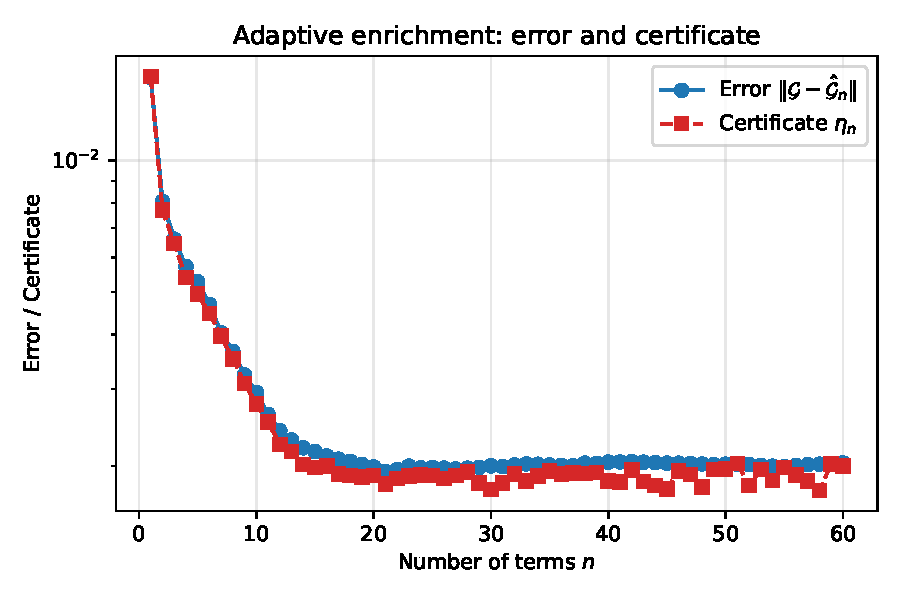
\includegraphics[width=0.47\textwidth]{figures/fig1_error_convergence.pdf}
\qquad
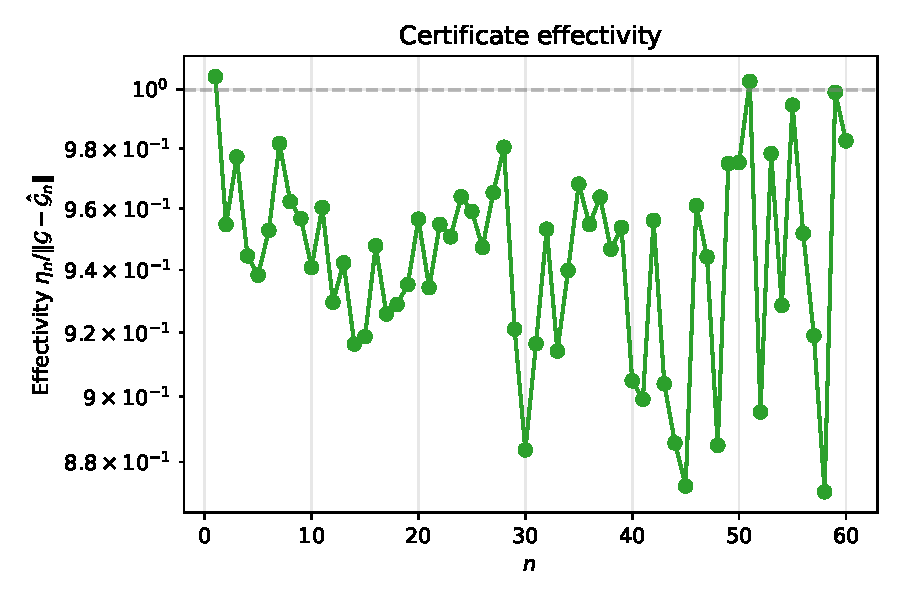
\includegraphics[width=0.47\textwidth]{figures/fig2_effectivity.pdf}
\caption{Left: adaptive enrichment convergence -- the true error $\|\calG-\wh\calG_n\|$ (blue) and the certificate $\eta_n$ (red dashed). Right: effectivity $\eta_n/\|\calG-\wh\calG_n\|$ throughout the enrichment. The certificate tracks the error closely, remaining within a factor~1 of the true error.}
\label{fig:convergence}
\end{figure}

\begin{figure}[t]
\centering
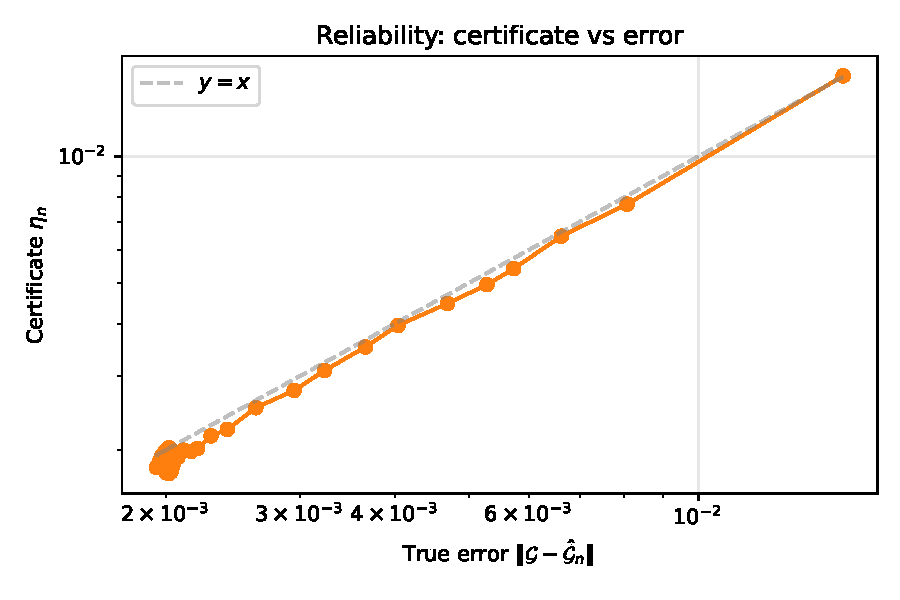
\includegraphics[width=0.47\textwidth]{figures/fig3_reliability.pdf}
\qquad
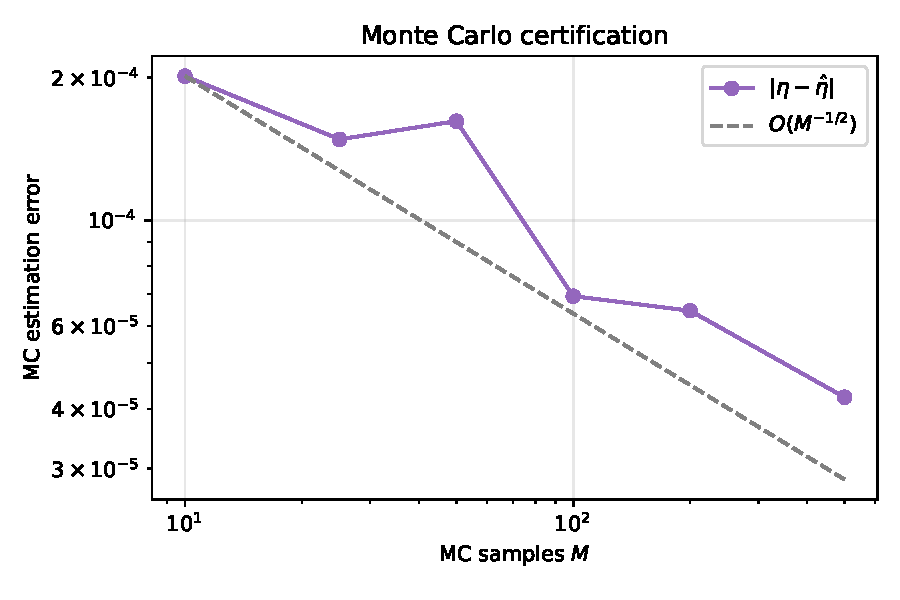
\includegraphics[width=0.47\textwidth]{figures/fig4_mc_convergence.pdf}
\caption{Left: certificate vs.\ true error (reliability plot). The points lie close to $y=x$, confirming the residual estimator provides an accurate upper bound. Right: Monte Carlo convergence of the statistical certificate. The empirical error (purple) follows the $O(M^{-1/2})$ reference line (gray dashed).}
\label{fig:reliability}
\end{figure}

%% ──────────────────────────────────────────────────────────────────────────────
\subsection{Regime of validity: slow parametric decay}
\label{sec:negative}
%% ──────────────────────────────────────────────────────────────────────────────

To assess the limitations of the framework, we consider a regime where the Karhunen--Lo\`{e}ve eigenvalues decay slowly as $\lambda_k\sim k^{-0.5}$ (compared to $k^{-2}$ in the baseline), with perturbation amplitude $\sigma=1.0$ and mean field $a_0=3$.
This models a random field with short correlation length, where the operator manifold has poor Kolmogorov width decay.
Table~\ref{tab:comparison} summarizes the results.

\begin{table}[t]
\centering
\caption{Comparison of the baseline and slow-KL regimes. The slow decay causes enrichment to stall and increases the cost of certification.}
\label{tab:comparison}
\begin{tabular}{lcc}
\toprule
Metric & Baseline ($k^{-2}$) & Slow KL ($k^{-0.5}$) \\
\midrule
Coercivity $\alpha$            & 0.8145 & 0.9092 \\
Final error                    & $2.03\times10^{-3}$ & $3.08\times10^{-2}$ \\
Error reduction (initial to final) & $7.5\times$ & $1.8\times$ \\
Certificate effectivity        & 0.98   & 0.82 \\
MC error at $M=500$            & $4.2\times10^{-5}$ & $3.7\times10^{-4}$ \\
Enrichment behaviour           & Continues & Stalls at $n\approx20$ \\
\bottomrule
\end{tabular}
\end{table}

Three effects are observed:
\begin{enumerate}
\item \textbf{Stalled enrichment:} the weak-greedy algorithm reduces the error by only a factor~1.8 before stalling, compared to $7.5\times$ in the baseline.
This is consistent with Assumption~\ref{ass:width}: the widths $d_n(\calM)_V$ decay too slowly for the polynomial chaos basis to achieve further reduction.
\item \textbf{Increased MC cost:} the Monte Carlo estimation error at $M=500$ is $3.7\times10^{-4}$, an order of magnitude larger than in the baseline, because the residual variance is higher.
The boundedness constant $B$ in Assumption~\ref{ass:bounded} is approximately $9.6\times10^{-3}$, about $15\times$ larger than the squared certificate value.
This translates to a proportional increase in the number of MC samples required to achieve a given statistical accuracy.
\item \textbf{Certificate reliability is preserved:} despite the degraded approximation, the certificate continues to track the error ($\eta_n/\|\calG-\wh\calG_n\|\approx0.8$).
The reliability bound (Lemma~\ref{thm:reliability}) holds regardless of the approximation quality.
\end{enumerate}

These findings delineate the regime where the present framework is most effective: problems with moderate-width operator manifolds, where the adaptive enrichment can achieve substantial error reduction and the statistical certification cost is controlled.
For problems with intrinsically slow width decay, the framework correctly identifies that the approximation is poor (via the certificate) but the remedy must come from a richer hypothesis class or a different architecture.

\begin{figure}[t]
\centering
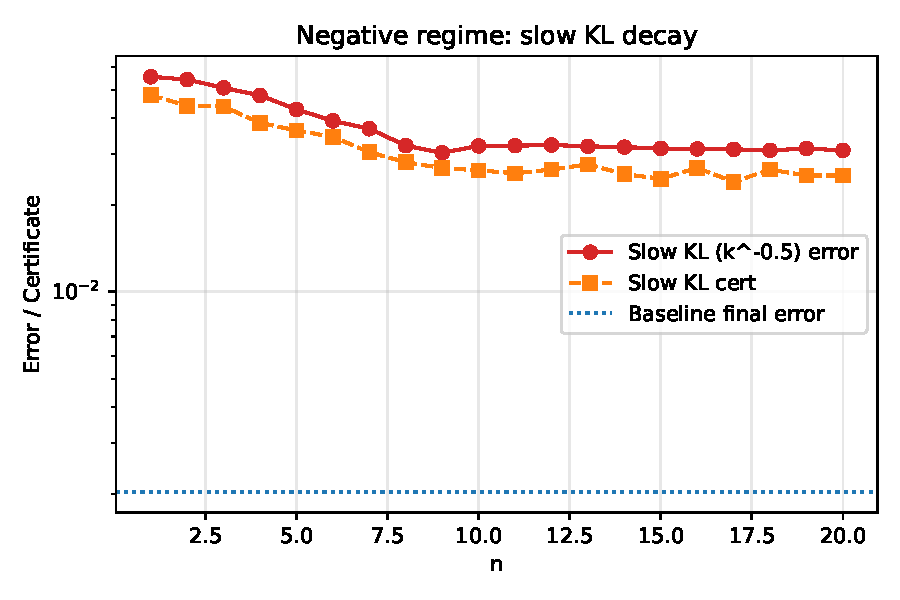
\includegraphics[width=0.47\textwidth]{figures/fig5_slow_kl_convergence.pdf}
\qquad
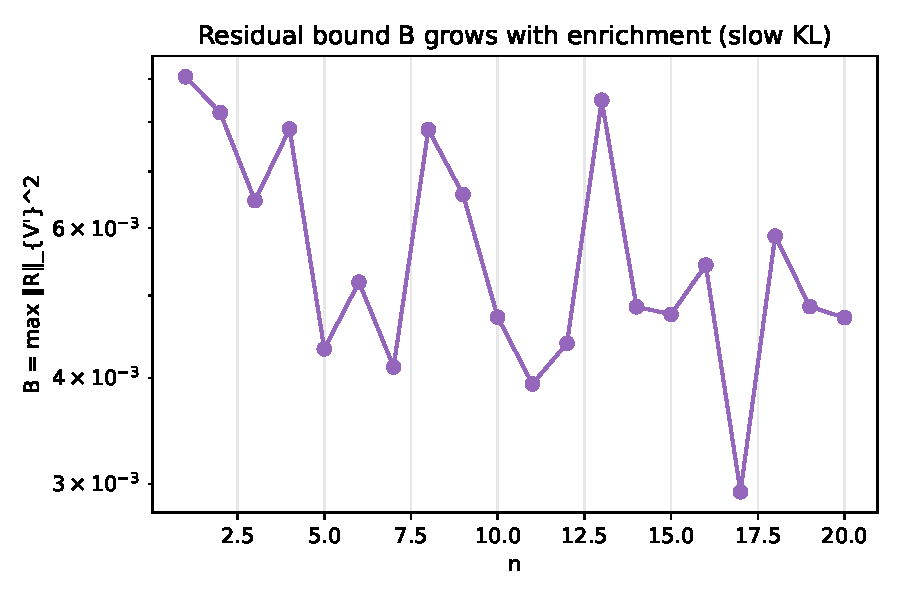
\includegraphics[width=0.47\textwidth]{figures/fig6_B_growth.pdf}
\caption{Left: error and certificate for the slow-KL regime ($k^{-0.5}$). The enrichment stalls after 20 steps, with error only dropping $1.8\\times$ compared to $7.5\\times$ in the baseline. Right: the bound $B=\\max\\|R\\|_{V'}^2$ on the residual norm as enrichment progresses.}
\label{fig:slow}
\end{figure}

%% ══════════════════════════════════════════════════════════════════════════════
\section{Discussion and outlook}
\label{sec:outlook}
%% ══════════════════════════════════════════════════════════════════════════════

We have introduced a certification framework for adaptive operator learning that combines residual-based reliability, weak-greedy approximation rates, and statistical certification.
The framework is architecture-independent and provides an operator-learning analogue of the reliability and optimality theory of AFEM.

Several directions remain open.

\textbf{Architecture-specific rates.}
The width-based analysis gives an abstract rate $n^{-s}$.
For specific architectures—tensor trains, DeepONets, sparse polynomial expansions—one can prove that the Kolmogorov widths are realized with concrete complexity estimates.
This is the subject of a follow-up paper.

\textbf{Efficiency.}
The present framework provides only reliability (upper bound).
An efficiency bound $\eta_n\le C\|\calG-\wh\calG_n\|$ under appropriate saturation assumptions would provide a fully computable two-sided estimate and is a natural next step.

\textbf{Nonlinear operators.}
The extension to monotone nonlinear operators preserves the residual-error relationship~\cite{zeidler1990nonlinear} and will be treated in a separate paper.

\textbf{Computational complexity.}
A refined analysis of the total work $W(\varepsilon)$ to achieve error $\le\varepsilon$, balancing $n$ (approximation dimension) and $M_n$ (sample size), is an important practical question.
The optimal balance $M_n\sim n^{2s}$ (to make $\delta_n\sim n^{-s}$) suggests a specific sample size schedule.

\textbf{Adversarial parameter regimes.}
When the Kolmogorov widths decay slowly (e.g.\ for random fields with short correlation length), the certification becomes loose or requires excessive sampling.
Understanding this boundary is essential for practical deployment.

%% ══════════════════════════════════════════════════════════════════════════════
\bibliographystyle{plain}
\bibliography{references}
%% ══════════════════════════════════════════════════════════════════════════════

\end{document}
